\section{Introduction}

Large language models (LLMs) are increasingly used to perform analytical reasoning tasks across domains such as engineering, finance, governance, and scientific investigation. Despite rapid progress in model capabilities, a fundamental challenge remains: ensuring that analytical outputs produced by LLM-based systems maintain clear separation between machine-generated representations and human-grounded judgments.

The Foundational Reasoning and Feedback Protocol (FRFP) provides a structured framework for addressing this challenge. FRFP introduces a formal separation between \emph{explicit representations}, which are machine-manipulable artifacts, and \emph{tacit states}, which represent human competence, grounding, and endorsement. The protocol constrains reasoning systems so that machine processes operate strictly within explicit representation spaces while final acceptance or endorsement remains a human function.

The FRFP framework is developed through a multi-layer research program that spans theoretical foundations, formal validation, engineering translation, and empirical evaluation. The mathematical foundations of the framework are established in \emph{FRFPPaper Vol.~1}, which defines the explicit–tacit separation, the representational boundary, and the formal constraints governing reasoning protocols. A companion tutorial provides a pedagogical explanation of the underlying mathematics, while a formalization in the \emph{LEAN} theorem prover enables machine-checked validation of the theoretical structure.

Building on these foundations, \emph{FRFPPaper Vol.~2} develops a corpus of canonical case studies involving complex socio-technical failures. These case studies demonstrate how the FRFP framework can be applied to analyze real-world systems involving interactions between technical mechanisms, organizational processes, and governance structures.

The theoretical framework is translated into implementable procedures through the \emph{FRFP Technical Specification}. This specification converts the abstract protocol constraints into operational rules suitable for LLM-based reasoning pipelines, including explicit artifact discipline, navigation integrity, assumption quarantine, and separation between generation and endorsement.

Engineering-level descriptions of the protocol and its implications for AI reasoning systems are further developed through a series of FRFP white papers. These documents communicate the practical consequences of structured reasoning protocols for system design and illustrate how FRFP differs from traditional prompt-engineering approaches.

To empirically evaluate structured reasoning interventions, a general experimental framework is introduced in \emph{Experimental Methods for Evaluating AI Agents}. This framework defines controlled procedures for constructing frozen analytical tasks, generating comparable model outputs under different reasoning conditions, and performing blinded human evaluation of analytical artifacts.

Within this framework, the \emph{FRFP vs Base Survey} provides an empirical evaluation of protocol-guided reasoning. In this study, a set of historical socio-technical cases is analyzed under three conditions: baseline LLM analysis, protocol-guided LLM reasoning, and reconstructions derived from independent assessor reports. Model outputs are normalized into comparable artifacts and evaluated through blinded human comparison.

The survey relies on standardized one-page analytical summaries that present each model-generated analysis in a consistent format. These artifacts serve as the evaluation interface for human raters and allow direct comparison of reasoning outputs across experimental conditions.

Figure~\ref{fig:frfp_stack} summarizes the overall architecture of the FRFP research and validation program, illustrating how the theoretical, engineering, and empirical components interact.

\begin{figure}[t]
\centering
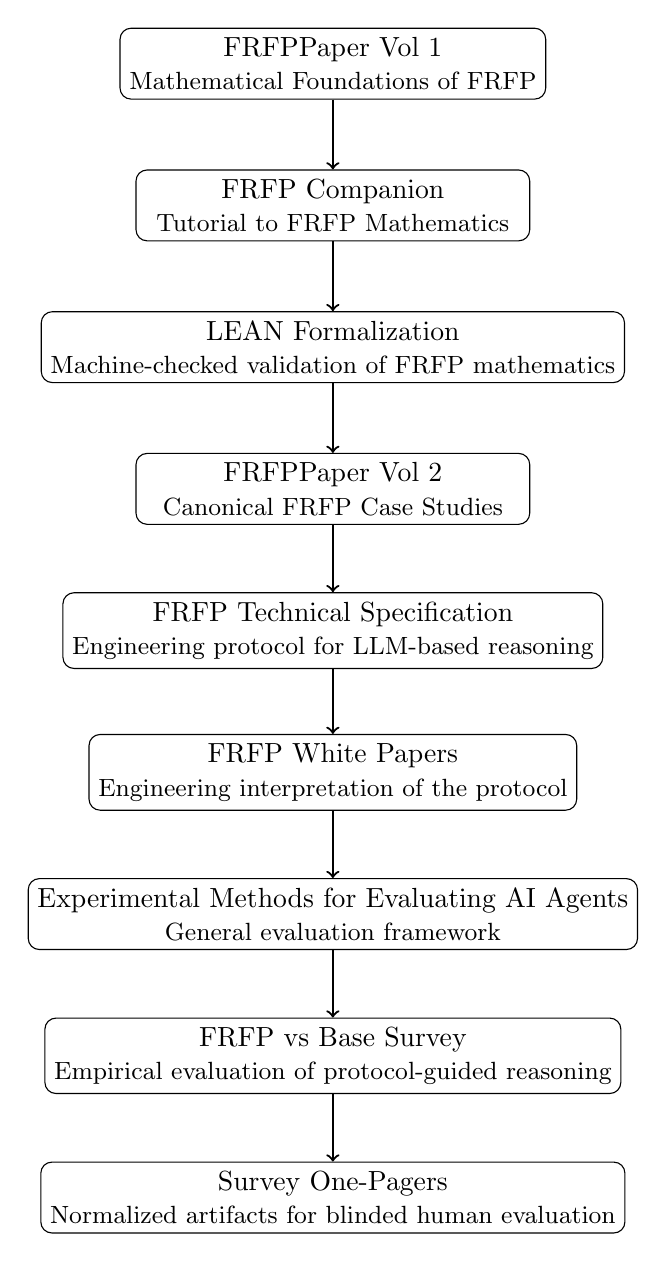
\begin{tikzpicture}[
node distance=1.8cm,
every node/.style={draw, rectangle, rounded corners, align=center, minimum width=5cm, minimum height=0.9cm},
arrow/.style={->, thick}
]

\node (vol1) {FRFPPaper Vol 1 \\ \small Mathematical Foundations of FRFP};

\node (companion) [below of=vol1] {FRFP Companion \\ \small Tutorial to FRFP Mathematics};

\node (lean) [below of=companion] {LEAN Formalization \\ \small Machine-checked validation of FRFP mathematics};

\node (vol2) [below of=lean] {FRFPPaper Vol 2 \\ \small Canonical FRFP Case Studies};

\node (techspec) [below of=vol2] {FRFP Technical Specification \\ \small Engineering protocol for LLM-based reasoning};

\node (whitepapers) [below of=techspec] {FRFP White Papers \\ \small Engineering interpretation of the protocol};

\node (methods) [below of=whitepapers] {Experimental Methods for Evaluating AI Agents \\ \small General evaluation framework};

\node (survey) [below of=methods] {FRFP vs Base Survey \\ \small Empirical evaluation of protocol-guided reasoning};

\node (onepagers) [below of=survey] {Survey One-Pagers \\ \small Normalized artifacts for blinded human evaluation};

\draw[arrow] (vol1) -- (companion);
\draw[arrow] (companion) -- (lean);
\draw[arrow] (lean) -- (vol2);
\draw[arrow] (vol2) -- (techspec);
\draw[arrow] (techspec) -- (whitepapers);
\draw[arrow] (whitepapers) -- (methods);
\draw[arrow] (methods) -- (survey);
\draw[arrow] (survey) -- (onepagers);

\end{tikzpicture}
\caption{FRFP research and validation stack. Mathematical foundations are translated into engineering protocols and evaluated through controlled experimental methodology and empirical survey analysis.}
\label{fig:frfp_stack}
\end{figure}

Together, these components establish a complete research pipeline for developing, implementing, and empirically evaluating structured reasoning protocols for AI-assisted analytical systems.

\begin{figure}[t]
\centering
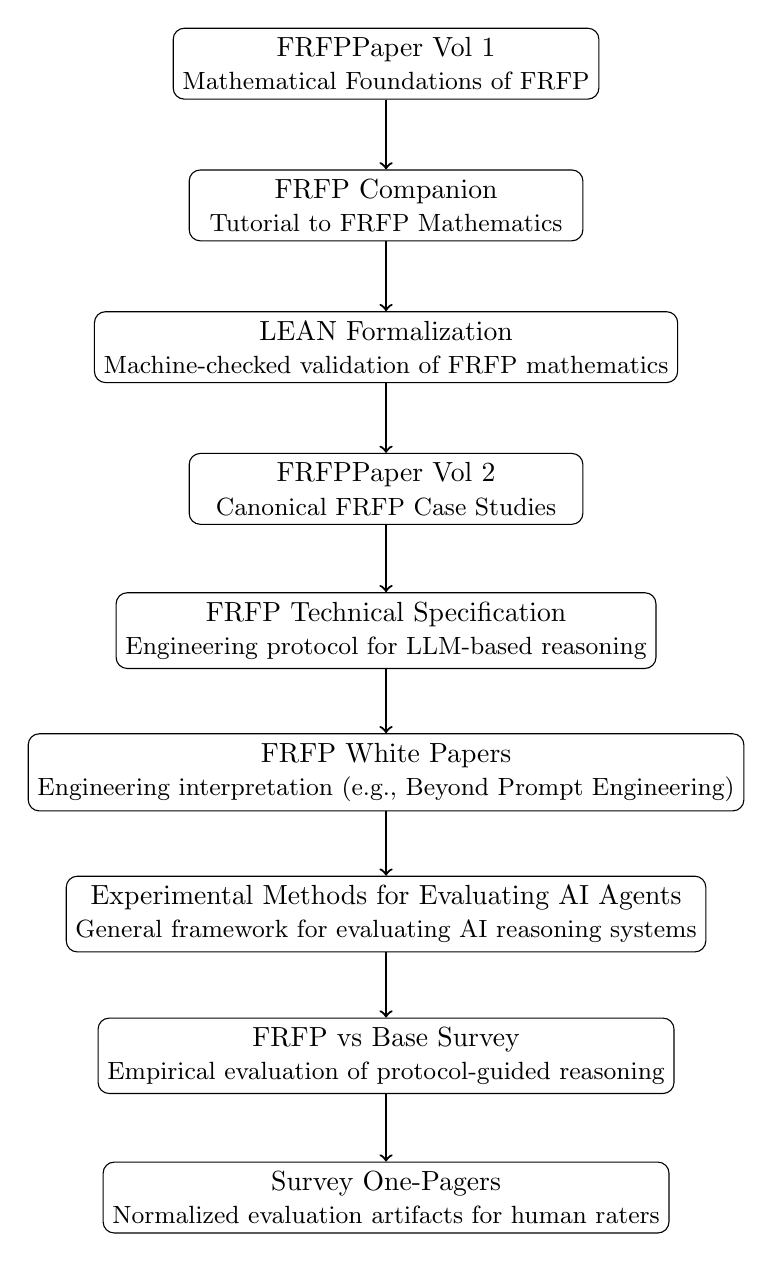
\begin{tikzpicture}[
node distance=1.8cm,
every node/.style={draw, rectangle, rounded corners, align=center, minimum width=5cm, minimum height=0.9cm},
arrow/.style={->, thick}
]

\node (vol1) {FRFPPaper Vol 1 \\ \small Mathematical Foundations of FRFP};

\node (companion) [below of=vol1] {FRFP Companion \\ \small Tutorial to FRFP Mathematics};

\node (lean) [below of=companion] {LEAN Formalization \\ \small Machine-checked validation of FRFP mathematics};

\node (vol2) [below of=lean] {FRFPPaper Vol 2 \\ \small Canonical FRFP Case Studies};

\node (techspec) [below of=vol2] {FRFP Technical Specification \\ \small Engineering protocol for LLM-based reasoning};

\node (whitepapers) [below of=techspec] {FRFP White Papers \\ \small Engineering interpretation (e.g., Beyond Prompt Engineering)};

\node (methods) [below of=whitepapers] {Experimental Methods for Evaluating AI Agents \\ \small General framework for evaluating AI reasoning systems};

\node (survey) [below of=methods] {FRFP vs Base Survey \\ \small Empirical evaluation of protocol-guided reasoning};

\node (onepagers) [below of=survey] {Survey One-Pagers \\ \small Normalized evaluation artifacts for human raters};

\draw[arrow] (vol1) -- (companion);
\draw[arrow] (companion) -- (lean);
\draw[arrow] (lean) -- (vol2);
\draw[arrow] (vol2) -- (techspec);
\draw[arrow] (techspec) -- (whitepapers);
\draw[arrow] (whitepapers) -- (methods);
\draw[arrow] (methods) -- (survey);
\draw[arrow] (survey) -- (onepagers);

\end{tikzpicture}
\caption{FRFP research and validation stack. Mathematical theory (top) is translated into engineering protocols and evaluated through controlled experimental methodology and empirical survey analysis.}
\end{figure}


\begin{figure*}[t]
\centering
\begin{tikzpicture}[
    font=\small,
    box/.style={
        draw,
        rounded corners=3pt,
        align=center,
        minimum height=0.95cm,
        text width=4.1cm,
        inner sep=6pt
    },
    layer/.style={
        draw,
        rounded corners=6pt,
        thick,
        inner sep=10pt
    },
    arr/.style={-{Latex[length=2.5mm]}, thick},
    darr/.style={-{Latex[length=2mm]}, semithick, dashed}
]

% --- THEORY LAYER ---
\node[layer, fill=blue!5, minimum width=14.2cm, minimum height=3.6cm] (theorybg) at (0,0) {};
\node[anchor=west, font=\bfseries\small] at (-6.8,1.45) {Theory Layer};

\node[box, fill=white] (vol1) at (-4.6,0.35)
{FRFPPaper Vol 1\\
\footnotesize Mathematical foundations of FRFP};

\node[box, fill=white] (companion) at (0,0.35)
{FRFP Companion\\
\footnotesize Tutorial to FRFP mathematics};

\node[box, fill=white] (lean) at (4.6,0.35)
{LEAN Validation\\
\footnotesize Machine-checked formalization of FRFP mathematics};

\draw[arr] (vol1) -- (companion);
\draw[arr] (companion) -- (lean);

% --- ENGINEERING LAYER ---
\node[layer, fill=green!6, minimum width=14.2cm, minimum height=4.2cm] (engbg) at (0,-4.4) {};
\node[anchor=west, font=\bfseries\small] at (-6.8,-2.55) {Engineering Layer};

\node[box, fill=white] (vol2) at (-4.6,-4.05)
{FRFPPaper Vol 2\\
\footnotesize Canonical FRFP case studies};

\node[box, fill=white] (techspec) at (0,-4.05)
{FRFP Technical Specification\\
\footnotesize Implementable protocol for LLM-based reasoning};

\node[box, fill=white] (whitepapers) at (4.6,-4.05)
{FRFP White Papers\\
\footnotesize Engineering descriptions of the protocol and its impact};

\draw[arr] (vol2) -- (techspec);
\draw[arr] (techspec) -- (whitepapers);

% --- EVALUATION LAYER ---
\node[layer, fill=orange!8, minimum width=14.2cm, minimum height=4.2cm] (evalbg) at (0,-9.0) {};
\node[anchor=west, font=\bfseries\small] at (-6.8,-7.15) {Evaluation Layer};

\node[box, fill=white] (methods) at (-4.6,-8.65)
{Experimental Methods for Evaluating AI Agents\\
\footnotesize General framework for controlled evaluation};

\node[box, fill=white] (survey) at (0,-8.65)
{FRFP vs Base Survey\\
\footnotesize Empirical evaluation of protocol-guided reasoning};

\node[box, fill=white] (onepagers) at (4.6,-8.65)
{Survey One-Pagers\\
\footnotesize Normalized artifacts for blinded human evaluation};

\draw[arr] (methods) -- (survey);
\draw[arr] (survey) -- (onepagers);

% --- VERTICAL FLOW BETWEEN LAYERS ---
\draw[arr] (companion.south) -- ++(0,-1.25) -| (techspec.north);
\draw[arr] (lean.south) -- ++(0,-1.1) -| (whitepapers.north);
\draw[arr] (techspec.south) -- ++(0,-1.25) -| (survey.north);
\draw[arr] (whitepapers.south) -- ++(0,-1.1) -| (methods.north);
\draw[darr] (vol2.south) -- ++(0,-1.15) -| (methods.north);

% --- OPTIONAL RIGHT-SIDE LABELS ---
\node[align=left, anchor=west, text width=2.7cm] at (7.6,0.35)
{\footnotesize
\textbf{Purpose:}\\
formal theory\\
pedagogy\\
mathematical validation};

\node[align=left, anchor=west, text width=2.7cm] at (7.6,-4.05)
{\footnotesize
\textbf{Purpose:}\\
case translation\\
engineering realization\\
practical interpretation};

\node[align=left, anchor=west, text width=2.7cm] at (7.6,-8.65)
{\footnotesize
\textbf{Purpose:}\\
general methodology\\
FRFP validation\\
human evaluation artifacts};

\end{tikzpicture}
\caption{Three-layer FRFP architecture. The theory layer defines the formal foundations of the framework and supports pedagogical and machine-checked validation. The engineering layer translates the theory into canonical case studies, implementable protocol specifications, and engineering-facing white papers. The evaluation layer provides a general experimental framework, an FRFP-specific empirical survey, and normalized one-page artifacts for blinded human assessment.}
\label{fig:frfp_three_layer_architecture}
\end{figure*}